\section{Brouillion}
\subsection*{Fluid formulation meaningful exchange terms}


Using the generic formulation \ref{eq:hybrid_avg_dt_chif} and the local expression of the mass, momentum and total energy expression, i.e. : \ref{eq:dt_rho},\ref{eq:dt_rhou_1} and \ref{eq:dt_rhoE_1} we easily find the averaged form of these equations as, 

\begin{align}
    \pddt (\phi_1 \rho_1)  
    + \div (
        \phi_1 \rho_1\textbf{u}_1
    )
    &= 
    0\\
    \pddt (\phi_1 \rho_1\textbf{u}_1)  
    + \div (
        \phi_1 \rho_1\textbf{u}_1\textbf{u}_1
        + \bm{\sigma}_1^\text{eq}
    )
    &= 
    \phi_1 \rho_1 \textbf{g} 
    -  \avg{\delta_I \bm{\sigma}_1^0 \cdot \textbf{n}_2}\\
    \pddt (\phi_1\rho_1E_1)  
    + \div (
        \phi_1\rho_1E_1\textbf{u}_1
        + \bm{q}_1^\text{eq}
        + \textbf{u}_1 \cdot \bm{\sigma}_1^\text{eq}
        % - \textbf{u}_1^0 \cdot \bm{\sigma}_1^0 
        % + \textbf{q}_1^0
        )
    &= 
    \phi_1 \rho_1\textbf{u}_1 \cdot \textbf{g} 
    - \avg{\delta_I (\textbf{u}_1^0 \cdot \bm{\sigma}_1^0 - \textbf{q}_1^0)\cdot \textbf{n}_2}
\end{align} 
where we have defined, 
\begin{align*}
    &\bm{\sigma}_1^\text{eq}
    = \phi_1 (
        \rho_1\kavg{\textbf{u}_1'\textbf{u}_1'}
        - \bm{\sigma}_1%- n_p \textbf{M}_p
         )  
    &\textbf{q}_1^\text{eq}
    =\textbf{q}_1^\text{e} +\textbf{q}_1^\text{k}  \\
    &\textbf{q}_1^\text{e}
    = \phi_1\rho_1 \kavg{\textbf{u}_1' e_1'} 
    + \phi_1\textbf{q}_1 
    &\textbf{q}_1^\text{k}
    = \phi_1\rho_1 \kavg{\textbf{u}_1' k_1} 
    - \phi_1\kavg{\textbf{u}_1' \cdot \bm{\sigma}_1^0}
\end{align*}
Note that the phase averaged energy equation can be further decompose following, 
\begin{align*}
    E_1 = e_1 + k_1 + u_1^2/2
    \label{eq:E_def}
\end{align*}
where $K_1$ is the pseudo-turbulent kinetic energy defined such as, $\phi_1 k_1 = \avg{\chi_1 (u_1')^2/2}$. 
The Macroscopic kinetic energy equation can be obtain by taking the dot product with $\textbf{u}_1$. 
\begin{align}
    \pddt (\phi_1 \rho_1u_1^2/2)  
    + \div (
        \phi_1 \rho_1\textbf{u}_1u_1^2/2
        + \textbf{u}_1 \cdot \bm{\sigma}_1^\text{eq}
    )
    &= 
     \bm{\sigma}_1^\text{eq} : \grad \textbf{u}_1
    + \phi_1 \rho_1 \textbf{u}_1\cdot \textbf{g} 
    -  \textbf{u}_1\cdot \avg{\delta_I \bm{\sigma}_1^0 \cdot \textbf{n}_2}\\
    \pddt (\phi_1\rho_1k_1)  
    + \div (
        \phi_1\rho_1k_1\textbf{u}_1
        + \textbf{q}_1^\text{k} 
        )
    &= 
    - \avg{\chi_1\bm{\sigma}_1^0 : \grad \textbf{u}_1^0}
    - \bm{\sigma}_1^\text{eq} : \grad \textbf{u}_1
    - \avg{\delta_I \textbf{u}_1' \cdot \bm{\sigma}_1^0 \cdot \textbf{n}_2}\\
    \pddt (\phi_1\rho_1e_1)  
    + \div (
        \phi_1 \rho_1e_1\textbf{u}_1
        +
        \textbf{q}_1^\text{e} 
        )
    &= 
    \avg{\chi_1\bm{\sigma}_1^0 : \grad \textbf{u}_1^0}
    + \avg{\delta_I \textbf{q}_1^0 \cdot \textbf{n}_2} 
\end{align}


Let's decompose the exchange term $\avg{\delta_I \textbf{u}^0_1 \cdot \bm{\sigma}_1^0 \cdot \textbf{n}_2}$.
The first step is to make appear the drag force term 
\begin{align*}
    \avg{\delta_I \textbf{u}^0_1 \cdot \bm{\sigma}_1^0 \cdot \textbf{n}_2}
    = 
    \avg{\delta_I \textbf{u}^0_2 \cdot \bm{\sigma}_1^0 \cdot \textbf{n}_2}
    =
    \textbf{u}_p \cdot  \avg{\delta_I \bm{\sigma}_1^0 \cdot \textbf{n}_2}
    % + \avg{\delta_I (\textbf{u}_\alpha - \textbf{u}_p) \cdot \bm{\sigma}_1^0 \cdot \textbf{n}_2}
    + \avg{\delta_I (\textbf{u}^0_2 - \textbf{u}_p) \cdot \bm{\sigma}_1^0 \cdot \textbf{n}_2}
\end{align*}
Maybe it is not the good way. In fact let first do that : 
\begin{align*}
    \avg{\delta_I \textbf{u}^0_1 \cdot \bm{\sigma}_1^0 \cdot \textbf{n}_2}
    =
    \pavg{ \intS{\textbf{u}^0_2 \cdot \bm{\sigma}_1^0 \cdot \textbf{n}_2}}
    - \div\pavg{ \intS{\textbf{r}\textbf{u}^0_2 \cdot \bm{\sigma}_1^0 \cdot \textbf{n}_2}}
\end{align*}
The first term can then be written as, 
\begin{align*}
    \pavg{ \intS{\textbf{u}^0_2 \cdot \bm{\sigma}_1^0 \cdot \textbf{n}_2}}
    = 
    \textbf{u}_p \cdot \pavg{\intS{\bm{\sigma}_1^0 \cdot \textbf{n}_2}}
    + \pavg{ \textbf{u}_\alpha' \cdot \intS{  \bm{\sigma}_1^0 \cdot \textbf{n}_2}}
    + \pavg{ \intS{\textbf{w}_2^0 \cdot \bm{\sigma}_1^0 \cdot \textbf{n}_2}}
\end{align*}
\begin{align*}
    \pavg{ \intS{\textbf{r}\textbf{u}^0_2 \cdot \bm{\sigma}_1^0 \cdot \textbf{n}_2}}
    = 
    \textbf{u}_p \cdot \pavg{\intS{ \textbf{r}\bm{\sigma}_1^0 \cdot \textbf{n}_2}}
    + \pavg{ \textbf{u}_\alpha' \cdot \intS{ \textbf{r} \bm{\sigma}_1^0 \cdot \textbf{n}_2}}
    + \pavg{ \intS{\textbf{r}\textbf{w}_2^0 \cdot \bm{\sigma}_1^0 \cdot \textbf{n}_2}}
\end{align*}
Here we have a proper decomposition into surface work etc.. 


Using this formulation we can say that, 
\begin{align}
    \label{eq:dt_avg_rho}
    &\pddt (\phi_1 \rho_1)  
    + \div (
        \phi_1 \rho_1\textbf{u}_1
    )
    = 
    0\\
    \label{eq:dt_avg_rhou_1}
    &\pddt (\phi_1 \rho_1\textbf{u}_1)  
    + \div (
        \phi_1 \rho_1\textbf{u}_1\textbf{u}_1
        + \bm{\sigma}_1^\text{eq}
    )
    = 
    \phi_1 \rho_1 \textbf{g} 
    - \pavg{\intS{\bm{\sigma}_1^0 \cdot \textbf{n}_2}}
    +\div  \pavg{\intS{\textbf{r}\bm{\sigma}_1^0 \cdot \textbf{n}_2}}
    \\
    \label{eq:dt_avg_rhoE_1}
    &\pddt (\phi_1\rho_1E_1)  
    + \div (
        \phi_1\rho_1E_1\textbf{u}_1
        + \bm{q}_1^\text{eq}
        + \textbf{u}_1 \cdot \bm{\sigma}_1^\text{eq}
        % - \textbf{u}_1^0 \cdot \bm{\sigma}_1^0 
        % + \textbf{q}_1^0
        )
    = 
    \phi_1 \rho_1\textbf{u}_1 \cdot \textbf{g} \\
    &- \textbf{u}_p \cdot \pavg{\intS{\bm{\sigma}_1^0 \cdot \textbf{n}_2}}
    - \pavg{ \textbf{u}_\alpha' \cdot \intS{  \bm{\sigma}_1^0 \cdot \textbf{n}_2}}
    - \pavg{ \intS{\textbf{w}_2^0 \cdot \bm{\sigma}_1^0 \cdot \textbf{n}_2}}
    + \pavg{\intS{\textbf{q}_1\cdot \textbf{n}_2}}
    % &\div [    
        % \textbf{u}_p \cdot \pavg{\intS{ \textbf{r}\bm{\sigma}_1^0 \cdot \textbf{n}_2}}
    % + \pavg{ \textbf{u}_\alpha' \cdot \intS{ \textbf{r} \bm{\sigma}_1^0 \cdot \textbf{n}_2}}
    % + \pavg{ \intS{\textbf{r}\textbf{w}_2^0 \cdot \bm{\sigma}_1^0 \cdot \textbf{n}_2}}
    % - \pavg{ \intS{\textbf{r}  \textbf{q}_1^0 \cdot \textbf{n}_2}}
    % ]
\end{align} 
where we have defined, 
\begin{align*}
    &\bm{\sigma}_1^\text{eq}
    = \phi_1 (
        \rho_1\kavg{\textbf{u}_1'\textbf{u}_1'}
        -\bm{\sigma}_1%- n_p \textbf{M}_p
        )  
        - \pavg{\intS{\textbf{r}\bm{\sigma}_1^0 \cdot \textbf{n}_2}}\\
    &\textbf{q}_1^\text{eq}
    =\textbf{q}_1^\text{e} +\textbf{q}_1^\text{k}  \\
    &\textbf{q}_1^\text{e}
    = \phi_1\rho_1 \kavg{\textbf{u}_1' e_1'} 
    + \phi_1\textbf{q}_1 
    +\pavg{\intS{\textbf{r}\textbf{q}_1^0 \cdot \textbf{n}_2}} 
    \\
    &\textbf{q}_1^\text{k}
    = \phi_1\rho_1 \kavg{\textbf{u}_1' k_1} 
    - \phi_1\kavg{\textbf{u}_1' \cdot \bm{\sigma}_1^0}
    + (\textbf{u}_1 - \textbf{u}_p)\cdot
    \pavg{\intS{\textbf{r}\bm{\sigma}_1^0 \cdot \textbf{n}_2}}
    \\
    &+ \pavg{ \textbf{u}_\alpha' \cdot \intS{ \textbf{r} \bm{\sigma}_1^0 \cdot \textbf{n}_2}}
    + \pavg{ \intS{\textbf{r}\textbf{w}_2^0 \cdot \bm{\sigma}_1^0 \cdot \textbf{n}_2}}
\end{align*}
Let's re derive the Secondary equations, firstly the kinetic energy equaitons, 
\begin{align*}
    \pddt (\phi_1 \rho_1u_1^2/2)  
    + \div (
        \phi_1 \rho_1\textbf{u}_1u_1^2/2
        + \textbf{u}_1 \cdot \bm{\sigma}_1^\text{eq}
    )
    &= 
     \bm{\sigma}_1^\text{eq} : \grad \textbf{u}_1
    + \phi_1 \rho_1 \textbf{u}_1\cdot \textbf{g} 
    -  \textbf{u}_1\cdot 
        \pavg{\intS{\bm{\sigma}_1^0 \cdot \textbf{n}_2}} 
        % - \div 
        % \pavg{\intS{\textbf{r}\bm{\sigma}_1^0 \cdot \textbf{n}_2}} 
        \\
    \pddt (\phi_1\rho_1k_1)  
    + \div (
        \phi_1\rho_1k_1\textbf{u}_1
        + \textbf{q}_1^\text{k} 
        )
    &= 
    - \avg{\chi_1\bm{\sigma}_1^0 : \grad \textbf{u}_1^0}
    - \bm{\sigma}_1^\text{eq} : \grad \textbf{u}_1\\
    &+ (\textbf{u}_1 - \textbf{u}_p)
    \cdot \pavg{\intS{\bm{\sigma}_1^0 \cdot \textbf{n}_2}}\\
    &- \pavg{ \textbf{u}_\alpha' \cdot \intS{  \bm{\sigma}_1^0 \cdot \textbf{n}_2}}
    - \pavg{ \intS{\textbf{w}_2^0 \cdot \bm{\sigma}_1^0 \cdot \textbf{n}_2}} 
    \\
    \pddt (\phi_1\rho_1e_1)  
    + \div (
        \phi_1 \rho_1e_1\textbf{u}_1
        +
        \textbf{q}_1^\text{e} 
        )
    &= 
    \avg{\chi_1\bm{\sigma}_1^0 : \grad \textbf{u}_1^0}
    + \pavg{\intS{\textbf{q}_1^0 \cdot \textbf{n}_2}} 
\end{align*}
The second equality here, gives in a homogeneous medium, 
\begin{equation*}
    0 =
    - \avg{\chi_1\bm{\sigma}_1^0 : \grad \textbf{u}_1^0}
    % - \bm{\sigma}_1^\text{eq} : \grad \textbf{u}_1
    + (\textbf{u}_1 - \textbf{u}_p)
    \cdot \pavg{\intS{\bm{\sigma}_1^0 \cdot \textbf{n}_2}}
    - \pavg{ \textbf{u}_\alpha' \cdot \intS{  \bm{\sigma}_1^0 \cdot \textbf{n}_2}}
    - \pavg{ \intS{\textbf{w}_2^0 \cdot \bm{\sigma}_1^0 \cdot \textbf{n}_2}} 
\end{equation*}
\subsection*{Particle formulation meaningful exchange terms}

For the dispersed phase we initially have :
\begin{align*}
    \pddt \left(n_p m_p\right)
    + \div \left(n_pm_p\textbf{u}_p
    \right)
    = 
    0\\
    \pddt \left(n_p m_p \textbf{u}_p\right)
    + \div \left(n_p
    m_p \textbf{u}_p \textbf{u}_p 
    + \bm{\sigma}_p^\text{eq}
    \right)
    = 
    n_p v_p \rho_2 \textbf{g}
    + n_p (\bm{\sigma}_1^0 \cdot \textbf{n}_2)_p^\Sigma,\\
    \pddt(m_p n_pE_p^\text{tot})
    + \div(m_pn_p E_p^\text{tot} \textbf{u}_p 
    + \textbf{q}_p^\text{eq} 
    + \textbf{u}_p \cdot \bm{\sigma}_p^\text{eq})
    =  n_p v_p \rho_2 \textbf{u}_p\cdot  \textbf{g}\\
    % +  n_p ( \textbf{u}'_1 \cdot \bm{\sigma}_1^0 \cdot \textbf{n}_2)_p^\Sigma
    -  n_p (\textbf{q}_1^0 \cdot \textbf{n}_2)_p^\Sigma
    + \textbf{u}_p \cdot\pavg{\intS{\bm{\sigma}_1^0 \cdot \textbf{n}_2}}
    + \pavg{\intS{\textbf{u}_\alpha' \cdot\bm{\sigma}_1^0 \cdot \textbf{n}_2}}
    + \pavg{\intS{\textbf{w}_2^0 \cdot\bm{\sigma}_1^0 \cdot \textbf{n}_2}}
\end{align*}
where we have defined, 
\begin{align*}
    &\bm{\sigma}_p^\text{eq}
    =  m_p\pnavg{\textbf{u}_\alpha'\textbf{u}_\alpha'}
    &\textbf{q}_p^\text{eq}
    =\textbf{q}_p^\text{e} 
    +\textbf{q}_p^\text{k}  
    +\textbf{q}_p^\text{w}  
    \\
    &\textbf{q}_1^\text{e}
    = m_p \pnavg{\textbf{u}_\alpha' e_\alpha'} 
    &\textbf{q}_p^\text{k}
    = m_p \pnavg{\textbf{u}_\alpha' k_\alpha} 
    \\
    &\textbf{q}_p^\text{w}
    = 
    + \pnavg{\textbf{u}_\alpha'(\rho_2 (w^0_2)^2/2 )'_\Omega}
    + \gamma \pnavg{\textbf{u}_\alpha' s_\alpha'}
\end{align*}
and, 
The exchange term of the energy equation can be rewritten as, 
\begin{equation*}
    \pavg{\intS{\textbf{u}_1^0\cdot\bm{\sigma}_1^0 \cdot \textbf{n}_2}}
    = 
    \textbf{u}_p \cdot\pavg{\intS{\bm{\sigma}_1^0 \cdot \textbf{n}_2}}
    + \pavg{\intS{\textbf{u}_\alpha' \cdot\bm{\sigma}_1^0 \cdot \textbf{n}_2}}
    + \pavg{\intS{\textbf{w}_2^0 \cdot\bm{\sigma}_1^0 \cdot \textbf{n}_2}}
\end{equation*}
Also, 
\begin{align*}
    &\pddt \left(n_p m_p u_p^2/ 2\right)
    + \div \left(n_p
    m_p u_p^2/ 2 \textbf{u}_p 
    + \textbf{u}_p \cdot \bm{\sigma}_p^\text{eq}
    \right)
    = 
    + \bm{\sigma}_p^\text{eq}  :\grad \textbf{u}_p
    +  n_p v_p \textbf{u}_p \cdot 
    \rho_2 \textbf{g}
    + n_p \textbf{u}_p \cdot (\bm{\sigma}_1^0 \cdot \textbf{n}_2)^\Sigma_p,\\
    &\pddt \left(n_p m_p (u_\alpha^2)_p/ 2\right)
    + \div \left(n_p
    m_p (u_\alpha^2)_p/ 2 \textbf{u}_p 
    + \textbf{q}^k_p
    + \textbf{u}_p \cdot \bm{\sigma}_p^\text{eq}
    \right)
    = 
    n_p m_p \textbf{u}_p \cdot
    \textbf{g}
    + \textbf{u}_p\cdot\pavg{\intS{\bm{\sigma}_1^0 \cdot \textbf{n}_2}}\\
    &+ \pavg{\textbf{u}_\alpha'\cdot\intS{\bm{\sigma}_1^0 \cdot \textbf{n}_2}}
    \\
    &\pddt \left(n_p W_p\right)
    + \div 
    (n_p W_p
    \textbf{u}_p 
    +  \textbf{q}_p^\text{w}
    )
    = 
    - n_p (\bm{\sigma}_2^0 : \grad\textbf{u}_2^0)^\Omega_p
    + n_p (\textbf{w}_2^0 \cdot \bm{\sigma}_1^0 \cdot  \textbf{n}_2)^\Sigma_p
    \\
    &\pddt \left(n_p m_p e_p\right)
    + \div \left(n_p
    m_p e_p \textbf{u}_p 
    +  \textbf{q}_p^\text{e}
    \right)
    = 
    + n_p (\bm{\sigma}_2^0 : \grad\textbf{u}_2^0)^\Omega_p
    - n_p (\textbf{q}_1^0\cdot \textbf{n}_2)^\Sigma_p\\
\end{align*}
The equaiton for $k_p$ reads, 
\begin{equation*}
    \pddt \left(n_p m_p k_p\right)
    + \div \left(n_p
    m_p k_p \textbf{u}_p 
    + \textbf{q}^k_p
    % + \textbf{u}_p \cdot \bm{\sigma}_p^\text{eq}
    \right)
    = 
    - \bm{\sigma}_p^\text{eq}  :\grad \textbf{u}_p
    + \pavg{\textbf{u}_\alpha'\cdot\intS{\bm{\sigma}_1^0 \cdot \textbf{n}_2}}
\end{equation*}
In agreement with kinetic theory without source term. 


Under this form the NRJ cascade takes the form
\begin{center}
    \tikzstyle{quadri}=[rectangle,draw]
    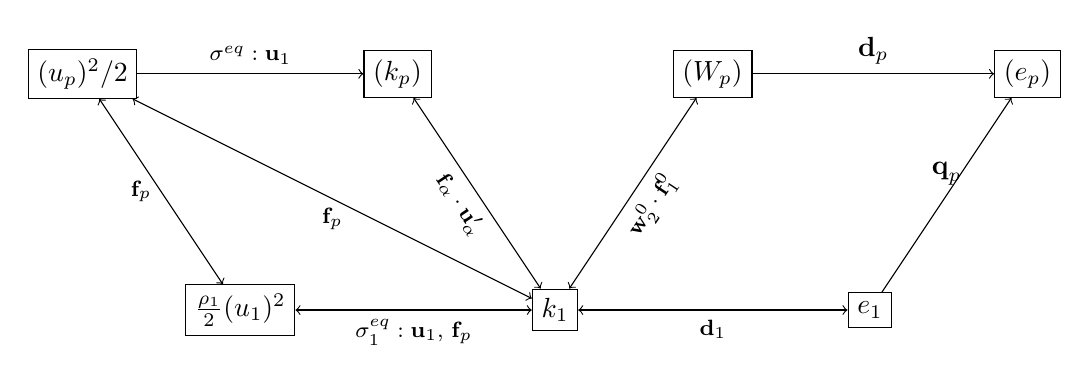
\begin{tikzpicture}
        \node[quadri] (u2) at (0,0){$(u_p)^2 / 2$};
        \node[quadri] (kp) at (4,0){$(k_p)$};
        \node[quadri] (Wp) at (8,0){$(W_p)$};
        \node[quadri] (ep) at (12,0){$(e_p)$};
        \node[quadri] (u12) at (2,-3){$\frac{\rho_1}{2}(u_1)^2$};
        \node[quadri] (k1) at (6,-3){$k_1$};
        \node[quadri] (e1) at (10,-3){$e_1$};
        \draw[->] (u2)--(kp)node[midway,above]{\footnotesize $\bm{\sigma}^\text{eq}:\grad \textbf{u}_1$};
        \draw[<->] (u2)--(u12) node[midway,left]{\footnotesize $\textbf{f}_{p} $};
        % \draw[<->,text width=2cm] (kp)--(u12) node[midway,left]{\footnotesize $+  n_p v_p \textbf{u}_p \cdot 
        % (\rho_2 \textbf{g} - \grad p_1)
        % + n_p \textbf{u}_p \cdot \textbf{f}_{pm} - \textbf{F}_\text{pfp}$};
        \draw[<->] (k1)--(u12) node[midway,below]{\footnotesize $\bm{\sigma}^\text{eq}_1:\grad \textbf{u}_1$, $\textbf{f}_p$};
        \draw[<->] (k1)--(e1) node[midway,below]{\footnotesize $\textbf{d}_1$};
        \draw[<->,sloped] (k1)--(kp) node[midway,below]{\footnotesize $\pavg{\textbf{f}_\alpha\cdot \textbf{u}_\alpha'}$};
        \draw[<->] (k1)--(u2) node[midway,below]{\footnotesize $\textbf{f}_p$};
        \draw[<->,sloped] (k1)--(Wp) node[midway,below]{\footnotesize $\pavg{\intS{\textbf{w}_2^0\cdot \textbf{f}_1^0}}$};
        % \draw[->] (kp)--(Wp)node[midway,above]{$(\textbf{u}_\alpha' \cdot \textbf{f}_\alpha')_p$};
        \draw[->] (Wp)--(ep)node[midway,above]{$\textbf{d}_p$};
        \draw[->] (e1)--(ep)node[midway,above]{$\textbf{q}_p$};
    \end{tikzpicture}
\end{center}

Thus, from this graph it is clear that the only way to makes the link between $k_p$ and the NRJ dissipation is through the addition of $k_p$ and $W_p$. Which gives, 
\begin{multline*}
    \pddt \left(n_p (W_p+m_p k_p)\right)
    + \div 
    (n_p (W_p+m_p k_p)
    \textbf{u}_p 
    +  \textbf{q}_p^\text{w}
    +  \textbf{q}_p^\text{k}
    )\\
    = 
    - n_p (\bm{\sigma}_2^0 : \grad\textbf{u}_2^0)^\Omega_p
    + n_p (\textbf{w}_2^0 \cdot \bm{\sigma}_1^0 \cdot  \textbf{n}_2)^\Sigma_p
    - \bm{\sigma}_p^\text{eq}  :\grad \textbf{u}_p
    + \pavg{\textbf{u}_\alpha'\cdot\intS{\bm{\sigma}_1^0 \cdot \textbf{n}_2}}
\end{multline*}
Here we recover the transfer terms of with the higher scales and the lower scales plus the ones of the fluid continuous phase...
In kinetic theory we consider non-slipping spherical particles such that the internal motion are constant, and non rotation is present.
In this situation it yields 
\begin{equation}
    \pddt \left(n_p m_p k_p\right)
    + \div 
    (n_p m_p k_p
    \textbf{u}_p 
    % +  \textbf{q}_p^\text{w}
    +  \textbf{q}_p^\text{k}
    )
    = 
    - n_p (\bm{\sigma}_2^0 : \grad\textbf{u}_2^0)^\Omega_p
    + n_p (\textbf{w}_2^0 \cdot \bm{\sigma}_1^0 \cdot  \textbf{n}_2)^\Sigma_p
    - \bm{\sigma}_p^\text{eq}  :\grad \textbf{u}_p
    + \pavg{\textbf{u}_\alpha'\cdot\intS{\bm{\sigma}_1^0 \cdot \textbf{n}_2}}
\end{equation}
Indeed, we still consider deformation inside the particles since a source term of dissipation is constant. 



\subsection{Inclusion of long range interactions}
\subsubsection*{Fluid phase}

Using this formulation we can say that, 
\begin{align}
    \label{eq:dt_avg_rho}
    &\pddt (\phi_1 \rho_1)  
    + \div (
        \phi_1 \rho_1\textbf{u}_1
    )
    = 
    0\\
    \label{eq:dt_avg_rhou_1}
    &\pddt (\phi_1 \rho_1\textbf{u}_1)  
    + \div (
        \phi_1 \rho_1\textbf{u}_1\textbf{u}_1
        + \bm{\sigma}_1^\text{eq}
    )
    = 
    \phi_1 \rho_1 \textbf{g} 
    % +  \pavg{\intS{\bm{\sigma}_1^0 \cdot \textbf{n}_2}}
    - n_p (\textbf{f}_\text{pm} + v_p \grad p_1)
    % +\div  \pavg{\intS{\textbf{r}\bm{\sigma}_1^0 \cdot \textbf{n}_2}}
    \\
    \label{eq:dt_avg_rhoE_1}
    &\pddt (\phi_1\rho_1E_1)  
    + \div (
        \phi_1\rho_1E_1\textbf{u}_1
        + \bm{q}_1^\text{eq}
        + \textbf{u}_1 \cdot \bm{\sigma}_1^\text{eq}
        % - \textbf{u}_1^0 \cdot \bm{\sigma}_1^0 
        % + \textbf{q}_1^0
        )
    = 
    \phi_1 \rho_1\textbf{u}_1 \cdot \textbf{g} 
    +n_p\textbf{F}_\text{pfp}:\grad \textbf{u}_p\\
    &
    - n_p \textbf{u}_p \cdot (\textbf{f}_\text{pm} + v_p \grad p_1)
    % \pavg{\intS{\bm{\sigma}_1^0 \cdot \textbf{n}_2}}
    - \pavg{ \textbf{u}_\alpha' \cdot \intS{  \bm{\sigma}_1^0 \cdot \textbf{n}_2}}
    - \pavg{ \intS{\textbf{w}_2^0 \cdot \bm{\sigma}_1^0 \cdot \textbf{n}_2}}
    + \pavg{\intS{\textbf{q}_1\cdot \textbf{n}_2}}
    % &\div [    
        % \textbf{u}_p \cdot \pavg{\intS{ \textbf{r}\bm{\sigma}_1^0 \cdot \textbf{n}_2}}
    % + \pavg{ \textbf{u}_\alpha' \cdot \intS{ \textbf{r} \bm{\sigma}_1^0 \cdot \textbf{n}_2}}
    % + \pavg{ \intS{\textbf{r}\textbf{w}_2^0 \cdot \bm{\sigma}_1^0 \cdot \textbf{n}_2}}
    % - \pavg{ \intS{\textbf{r}  \textbf{q}_1^0 \cdot \textbf{n}_2}}
    % ]
\end{align} 
where we have defined, 
\begin{align*}
    &\bm{\sigma}_1^\text{eq}
    = \phi_1 (
        \rho_1\kavg{\textbf{u}_1'\textbf{u}_1'}
        -\bm{\sigma}_1%- n_p \textbf{M}_p
        )  
        - \pavg{\intS{\textbf{r}\bm{\sigma}_1^0 \cdot \textbf{n}_2}}
        + \textbf{F}_\text{pfp}\\
    &\textbf{q}_1^\text{eq}
    =\textbf{q}_1^\text{e} +\textbf{q}_1^\text{k}  \\
    &\textbf{q}_1^\text{e}
    = \phi_1\rho_1 \kavg{\textbf{u}_1' e_1'} 
    + \phi_1\textbf{q}_1 
    +\pavg{\intS{\textbf{r}\textbf{q}_1^0 \cdot \textbf{n}_2}} 
    \\
    &\textbf{q}_1^\text{k}
    = \phi_1\rho_1 \kavg{\textbf{u}_1' k_1} 
    - \phi_1\kavg{\textbf{u}_1' \cdot \bm{\sigma}_1^0}
    + (\textbf{u}_1 - \textbf{u}_p)\cdot[
    \pavg{\intS{\textbf{r}\bm{\sigma}_1^0 \cdot \textbf{n}_2}}
     - n_p \textbf{F}_\text{pfp}]
    \\
    &+ \pavg{ \textbf{u}_\alpha' \cdot \intS{ \textbf{r} \bm{\sigma}_1^0 \cdot \textbf{n}_2}}
    + \pavg{ \intS{\textbf{r}\textbf{w}_2^0 \cdot \bm{\sigma}_1^0 \cdot \textbf{n}_2}}
\end{align*}
Let's re derive the Secondary equations, firstly the kinetic energy equaitons, 
\begin{align*}
    \pddt (\phi_1 \rho_1u_1^2/2)  
    + \div (
        \phi_1 \rho_1\textbf{u}_1u_1^2/2
        + \textbf{u}_1 \cdot \bm{\sigma}_1^\text{eq}
    )
    &= 
     \bm{\sigma}_1^\text{eq} : \grad \textbf{u}_1
    + \phi_1 \rho_1 \textbf{u}_1\cdot \textbf{g} 
    -  n_p \textbf{u}_1\cdot 
    (\textbf{f}_\text{pm} + v_1\grad p_1)
        % \pavg{\intS{\bm{\sigma}_1^0 \cdot \textbf{n}_2}} 
        % - \div 
        % \pavg{\intS{\textbf{r}\bm{\sigma}_1^0 \cdot \textbf{n}_2}} 
        \\
    \pddt (\phi_1\rho_1k_1)  
    + \div (
        \phi_1\rho_1k_1\textbf{u}_1
        + \textbf{q}_1^\text{k} 
        )
    &= 
    - \avg{\chi_1\bm{\sigma}_1^0 : \grad \textbf{u}_1^0}
    - \bm{\sigma}_1^\text{eq} : \grad \textbf{u}_1
    + n_p \textbf{F}_\text{pfp} : \grad \textbf{u}_p
    \\
    &+ n_p (\textbf{u}_1 - \textbf{u}_p)
    \cdot (\textbf{f}_\text{pm} - v_p \grad p_1)\\
    &- \pavg{ \textbf{u}_\alpha' \cdot \intS{  \bm{\sigma}_1^0 \cdot \textbf{n}_2}}
    - \pavg{ \intS{\textbf{w}_2^0 \cdot \bm{\sigma}_1^0 \cdot \textbf{n}_2}} 
    \\
    \pddt (\phi_1\rho_1e_1)  
    + \div (
        \phi_1 \rho_1e_1\textbf{u}_1
        +
        \textbf{q}_1^\text{e} 
        )
    &= 
    \avg{\chi_1\bm{\sigma}_1^0 : \grad \textbf{u}_1^0}
    + \pavg{\intS{\textbf{q}_1^0 \cdot \textbf{n}_2}} 
\end{align*}
The homogeneous equilibrium stays the same. 
\subsection*{Particle phase with pfp and dumped pressure}
On the particle phase


For the dispersed phase we initially have :
\begin{align*}
    \pddt \left(n_p m_p\right)
    + \div \left(n_pm_p\textbf{u}_p
    \right)
    = 
    0\\
    \pddt \left(n_p m_p \textbf{u}_p\right)
    + \div \left(n_p
    m_p \textbf{u}_p \textbf{u}_p 
    + \bm{\sigma}_p^\text{eq}
    \right)
    = 
    n_p v_p \rho_2 \textbf{g}
    + n_p (\textbf{f}_\text{pm} + v_p \grad p_1),
    \\
    \pddt(m_p n_pE_p^\text{tot})
    + \div(m_pn_p E_p^\text{tot} \textbf{u}_p 
    + \textbf{q}_p^\text{eq} 
    + \textbf{u}_p \cdot \bm{\sigma}_p^\text{eq})
    =  n_p v_p \rho_2 \textbf{u}_p\cdot  \textbf{g}
    % +  n_p ( \textbf{u}'_1 \cdot \bm{\sigma}_1^0 \cdot \textbf{n}_2)_p^\Sigma
    -  n_p (\textbf{q}_1^0 \cdot \textbf{n}_2)_p^\Sigma\\
    - n_p \textbf{F}_\text{pfp} : \grad \textbf{u}_p
    + \textbf{u}_p \cdot (\textbf{f}_\text{pm} + v_p\grad p_1)
    + \pavg{\intS{\textbf{u}_\alpha' \cdot\bm{\sigma}_1^0 \cdot \textbf{n}_2}}
    + \pavg{\intS{\textbf{w}_2^0 \cdot\bm{\sigma}_1^0 \cdot \textbf{n}_2}}
\end{align*}
where we have defined, 
\begin{align*}
    &\bm{\sigma}_p^\text{eq}
    =  m_p\pnavg{\textbf{u}_\alpha'\textbf{u}_\alpha'}
    - n_p \textbf{F}_\text{pfp}
    &\textbf{q}_p^\text{eq}
    =\textbf{q}_p^\text{e} 
    +\textbf{q}_p^\text{k}  
    +\textbf{q}_p^\text{w}  
    \\
    &\textbf{q}_1^\text{e}
    = m_p \pnavg{\textbf{u}_\alpha' e_\alpha'} 
    &\textbf{q}_p^\text{k}
    = m_p \pnavg{\textbf{u}_\alpha' k_\alpha} 
    \\
    &\textbf{q}_p^\text{w}
    = 
    + \pnavg{\textbf{u}_\alpha'(\rho_2 (w^0_2)^2/2 )'_\Omega}
    + \gamma \pnavg{\textbf{u}_\alpha' s_\alpha'}
\end{align*}
Also, 
\begin{align*}
    &\pddt \left(n_p m_p u_p^2/ 2\right)
    + \div \left(n_p
    m_p u_p^2/ 2 \textbf{u}_p 
    + \textbf{u}_p \cdot \bm{\sigma}_p^\text{eq}
    \right)
    = 
    + \bm{\sigma}_p^\text{eq}  :\grad \textbf{u}_p
    +  n_p v_p \textbf{u}_p \cdot 
    \rho_2 \textbf{g}
    + n_p \textbf{u}_p \cdot (\textbf{f}_\text{pm} + v_p \grad p_1),\\
    &\pddt \left(n_p m_p (u_\alpha^2)_p/ 2\right)
    + \div \left(n_p
    m_p (u_\alpha^2)_p/ 2 \textbf{u}_p 
    + \textbf{q}^k_p
    + \textbf{u}_p \cdot \bm{\sigma}_p^\text{eq}
    \right)
    = 
    n_p m_p \textbf{u}_p \cdot
    \textbf{g}
    + \textbf{u}_p\cdot(\textbf{f}_\text{pm} + v_p \grad p_1)\\
    &- n_p \textbf{F}_\text{pfp} : \grad \textbf{u}_p
    + \pavg{\textbf{u}_\alpha'\cdot\intS{\bm{\sigma}_1^0 \cdot \textbf{n}_2}}
    \\
    &\pddt \left(n_p W_p\right)
    + \div 
    (n_p W_p
    \textbf{u}_p 
    +  \textbf{q}_p^\text{w}
    )
    = 
    - n_p (\bm{\sigma}_2^0 : \grad\textbf{u}_2^0)^\Omega_p
    + n_p (\textbf{w}_2^0 \cdot \bm{\sigma}_1^0 \cdot  \textbf{n}_2)^\Sigma_p
    \\
    &\pddt \left(n_p m_p e_p\right)
    + \div \left(n_p
    m_p e_p \textbf{u}_p 
    +  \textbf{q}_p^\text{e}
    \right)
    = 
    + n_p (\bm{\sigma}_2^0 : \grad\textbf{u}_2^0)^\Omega_p
    - n_p (\textbf{q}_1^0\cdot \textbf{n}_2)^\Sigma_p\\
\end{align*}
The equaiton for $k_p$ reads, 
\begin{equation*}
    \pddt \left(n_p m_p k_p\right)
    + \div \left(n_p
    m_p k_p \textbf{u}_p 
    + \textbf{q}^k_p
    % + \textbf{u}_p \cdot \bm{\sigma}_p^\text{eq}
    \right)
    = 
    - \pavg{\textbf{u}_\alpha'\textbf{u}_\alpha'} :\grad \textbf{u}_p
    + \pavg{\textbf{u}_\alpha'\cdot\intS{\bm{\sigma}_1^0 \cdot \textbf{n}_2}}
\end{equation*}
In agreement with kinetic theory without source term. 


Under this form the NRJ cascade takes the form
\begin{center}
    \tikzstyle{quadri}=[rectangle,draw]
    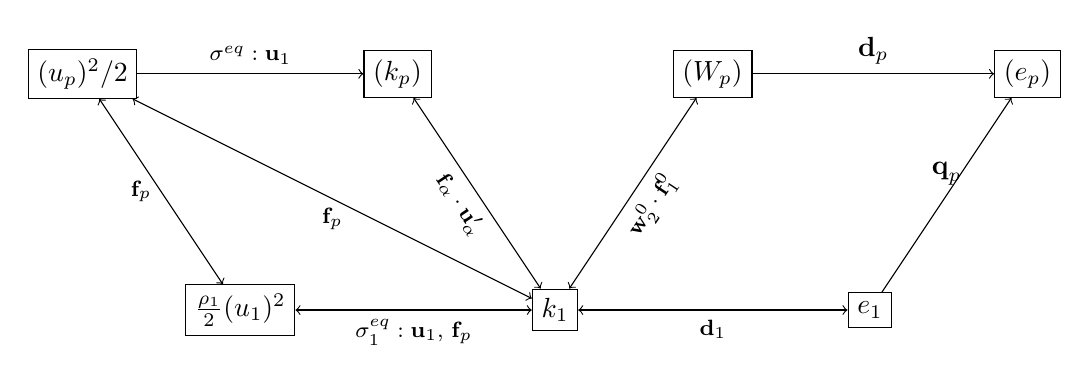
\begin{tikzpicture}
        \node[quadri] (u2) at (0,0){$(u_p)^2 / 2$};
        \node[quadri] (kp) at (4,0){$(k_p)$};
        \node[quadri] (Wp) at (8,0){$(W_p)$};
        \node[quadri] (ep) at (12,0){$(e_p)$};
        \node[quadri] (u12) at (2,-3){$\frac{\rho_1}{2}(u_1)^2$};
        \node[quadri] (k1) at (6,-3){$k_1$};
        \node[quadri] (e1) at (10,-3){$e_1$};
        \draw[->] (u2)--(kp)node[midway,above]{\footnotesize $\bm{\sigma}^\text{eq}:\grad \textbf{u}_1$};
        \draw[<->] (u2)--(u12) node[midway,left]{\footnotesize $\textbf{f}_{p} $};
        % \draw[<->,text width=2cm] (kp)--(u12) node[midway,left]{\footnotesize $+  n_p v_p \textbf{u}_p \cdot 
        % (\rho_2 \textbf{g} - \grad p_1)
        % + n_p \textbf{u}_p \cdot \textbf{f}_{pm} - \textbf{F}_\text{pfp}$};
        \draw[<->] (k1)--(u12) node[midway,below]{\footnotesize $\bm{\sigma}^\text{eq}_1:\grad \textbf{u}_1$, $\textbf{f}_p$};
        \draw[<->] (k1)--(e1) node[midway,below]{\footnotesize $\textbf{d}_1$};
        \draw[<->,sloped] (k1)--(kp) node[midway,below]{\footnotesize $\pavg{\textbf{f}_\alpha\cdot \textbf{u}_\alpha'}$};
        \draw[<->] (k1)--(u2) node[midway,below]{\footnotesize $\textbf{f}_p$};
        \draw[<->,sloped] (k1)--(Wp) node[midway,below]{\footnotesize $\pavg{\intS{\textbf{w}_2^0\cdot \textbf{f}_1^0}}$};
        % \draw[->] (kp)--(Wp)node[midway,above]{$(\textbf{u}_\alpha' \cdot \textbf{f}_\alpha')_p$};
        \draw[->] (Wp)--(ep)node[midway,above]{$\textbf{d}_p$};
        \draw[->] (e1)--(ep)node[midway,above]{$\textbf{q}_p$};
    \end{tikzpicture}
\end{center}

Thus, from this graph it is clear that the only way to makes the link between $k_p$ and the NRJ dissipation is through the addition of $k_p$ and $W_p$. Which gives, 
\begin{multline*}
    \pddt \left(n_p (W_p+m_p k_p)\right)
    + \div 
    (n_p (W_p+m_p k_p)
    \textbf{u}_p 
    +  \textbf{q}_p^\text{w}
    +  \textbf{q}_p^\text{k}
    )\\
    = 
    - n_p (\bm{\sigma}_2^0 : \grad\textbf{u}_2^0)^\Omega_p
    + n_p (\textbf{w}_2^0 \cdot \bm{\sigma}_1^0 \cdot  \textbf{n}_2)^\Sigma_p
    - \bm{\sigma}_p^\text{eq}  :\grad \textbf{u}_p
    + \pavg{\textbf{u}_\alpha'\cdot\intS{\bm{\sigma}_1^0 \cdot \textbf{n}_2}}
\end{multline*}
Here we recover the transfer terms of with the higher scales and the lower scales plus the ones of the fluid continuous phase...
In kinetic theory we consider non-slipping spherical particles such that the internal motion are constant, and non rotation is present.
In this situation it yields 
\begin{equation}
    \pddt \left(n_p m_p k_p\right)
    + \div 
    (n_p m_p k_p
    \textbf{u}_p 
    % +  \textbf{q}_p^\text{w}
    +  \textbf{q}_p^\text{k}
    )
    = 
    - n_p (\bm{\sigma}_2^0 : \grad\textbf{u}_2^0)^\Omega_p
    + n_p (\textbf{w}_2^0 \cdot \bm{\sigma}_1^0 \cdot  \textbf{n}_2)^\Sigma_p
    - \bm{\sigma}_p^\text{eq}  :\grad \textbf{u}_p
    + \pavg{\textbf{u}_\alpha'\cdot\intS{\bm{\sigma}_1^0 \cdot \textbf{n}_2}}
\end{equation}
Indeed, we still consider deformation inside the particles since a source term of dissipation is constant. 

